\documentclass[a4paper,10pt]{scrartcl}

\usepackage{graphicx}
\usepackage[utf8]{inputenc}
\usepackage{url}
\usepackage{xspace}
\usepackage[left=20mm,top=20mm]{geometry}
\usepackage{algorithmic}
\usepackage{subcaption}
\usepackage{mathpazo}
\usepackage{booktabs}
\usepackage{hyperref}
\usepackage{tabularx}

\usepackage{amsmath,amssymb,amsthm} 
\usepackage{physics}
% \usepackage{draftwatermark}

\newcommand{\ie}{ie}
\newcommand{\eg}{eg}
\newcommand{\reffig}[1]{Figure~\ref{#1}}
\newcommand{\refsec}[1]{Section~\ref{#1}}

\setcapindent{1em} %-- for captions of Figures

\renewcommand{\algorithmicrequire}{\textbf{Input:}}
\renewcommand{\algorithmicensure}{\textbf{Output:}}


\title{Quantum Computing Cheat Sheet}

\author{Valentin Taillandier}

\begin{document}

\maketitle

%%%

\section*{State vectors}
\[\ket{\psi} = \begin{pmatrix}
\cos \frac{\theta}{2}\\ 
e^{i \varphi } \sin \frac{\theta}{2}
\end{pmatrix}\]


\begin{minipage}{\linewidth}
\begin{minipage}{0.5\linewidth}
\[\ket{0} = \begin{pmatrix}
1 \\
0
\end{pmatrix}\]
\[\ket{\text{+}} = \frac{\ket{0} + \ket{1}}{\sqrt{2}}\]
\[\ket{\text{+}'} = \frac{\ket{0} + i\ket{1}}{\sqrt{2}}\]

\end{minipage}
\begin{minipage}{0.5\linewidth}
\[\ket{1} = \begin{pmatrix}
0 \\
1
\end{pmatrix}\]
\[\ket{\text{-}} = \frac{\ket{0} - \ket{1}}{\sqrt{2}}\]
\[\ket{\text{-}'} = \frac{\ket{0} - i\ket{1}}{\sqrt{2}}\]
\end{minipage}
\end{minipage}


\section*{Bloch sphere}


\begin{minipage}{\linewidth}

\begin{minipage}{0.5\linewidth}\center
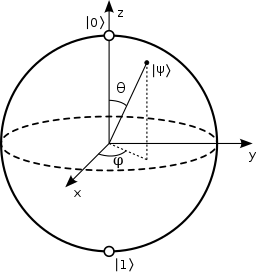
\includegraphics[scale=0.5]{img/bloch.png}
\end{minipage}
\begin{minipage}{0.5\linewidth}\center
\[ \begin{pmatrix}
r_x \\
r_y \\
r_z
\end{pmatrix}
=
\begin{pmatrix}
\sin \theta \cos \varphi \\
\sin \theta \sin \varphi \\
\cos \theta
\end{pmatrix}
\]
\end{minipage}
\end{minipage}



\section*{Pauli matrices}

\begin{center}


$
X = 
\begin{pmatrix}
0 & 1 \\ 
1 & 0 
\end{pmatrix}
$
\hspace{0.1\linewidth}
$
Y = 
\begin{pmatrix}
0 & -i \\ 
i & 0 
\end{pmatrix}
$
\hspace{0.1\linewidth}
$
Z = 
\begin{pmatrix}
1 & 0 \\ 
0 & -1 
\end{pmatrix}
$
\end{center}
\vspace{2\baselineskip}
\begin{minipage}{\linewidth}
\begin{minipage}{0.5\linewidth}\center

\begin{tabular}{c|c|c|c|}
\cline{2-4}
$\Rsh\times$                  & $X$   & $Y$   & $Z$   \\ \hline
\multicolumn{1}{|c|}{$X$} & $I$   & $iZ$  & $-iY$ \\ \hline
\multicolumn{1}{|c|}{$Y$} & $-iZ$ & $I$   & $iX$  \\ \hline
\multicolumn{1}{|c|}{$Z$} & $iY$  & $-iX$ & $I$   \\ \hline
\end{tabular}

\end{minipage}
\begin{minipage}{0.5\linewidth}
\begin{equation*}
\begin{split}
X &= \ket{\text{+}}\bra{+} - \ket{\text{-}}\bra{\text{-}}\\
Y &= \ket{\text{+}'}\bra{\text{+}'} - \ket{\text{-}'}\bra{\text{-}'}\\
Z &= \ket{0}\bra{0} - \ket{1}\bra{1}\\
\end{split}
\end{equation*}
\end{minipage}
\end{minipage}

\section*{Rotations}

\begin{equation*}
\begin{split}
R_x(\theta) &= e^{-i\theta X /2} = \cos{\frac{\theta}{2}}I - i\sin{\frac{\theta}{2}}X \\
R_y(\theta) &= e^{-i\theta Y /2} = \cos{\frac{\theta}{2}}I - i\sin{\frac{\theta}{2}}Y \\
R_z(\theta) &= e^{-i\theta Z /2} = \cos{\frac{\theta}{2}}I - i\sin{\frac{\theta}{2}}Z \\
\end{split}
\end{equation*}

\section*{Density matrix}
\[\rho = \ket{\psi}\bra{\psi}\]
\[\rho = \frac{1}{2}(I + \sin \theta \cos \varphi X + \sin \theta \sin \varphi Y + \cos \theta Z)\]
\[\rho = \frac{1}{2}(I + r_x X +  r_y Y + r_z Z)\]
\\
$\psi$ is a pure-state $\Leftrightarrow Tr(\rho ^ 2) = 1 \Leftrightarrow r_x^2+ r_y^2 + r_z^2 = 1$

\section*{Tomography}

\begin{equation*}
\begin{split}
r_x &= Tr(X\rho) = \bra{\text{+}}{\rho} \ket{\text{+}} - \bra{\text{-}}{\rho} \ket{\text{-}} = \mathbb{P}\ket{\text{+}}-\mathbb{P}\ket{\text{-}}\\
r_y &= Tr(Y\rho) = \bra{\text{+}'}{\rho} \ket{\text{+}'} - \bra{\text{-}'}{\rho} \ket{\text{-}'} = \mathbb{P}\ket{\text{+}'}-\mathbb{P}\ket{\text{-}'}\\
r_z &= Tr(Z\rho) = \bra{0}{\rho} \ket{0} - \bra{1}{\rho} \ket{1} = \mathbb{P}\ket{0}-\mathbb{P}\ket{1}
\end{split}
\end{equation*}

\section*{Gates}
\subsection*{Hadamard Gate}
The Hadamard Gate can be decomposed in two rotations:
\[H = 
\frac{1}{\sqrt{2}}\begin{pmatrix}
1 & 1\\ 
1 & -1
\end{pmatrix}
= \ket{\text{+}}\bra{0} + \ket{\text{-}}\bra{1}
= R_x(\pi)R_y(\frac{\pi}{2}) = -iX \cdot R_y(\frac{\pi}{2}) 
\]

\subsection*{Phase Gate}
\[S = 
\begin{pmatrix}
1 & 0\\ 
0 & i
\end{pmatrix}
= \ket{0}\bra{0} + i\ket{\text{1}}\bra{1}
\]



\subsection*{Controlled Not (CNOT, CX)}


\begin{minipage}{\linewidth}
\begin{minipage}{0.5\linewidth}\center
\[CX = 
\begin{pmatrix}
1 & 0 & 0 & 0\\ 
0 & 1 & 0 & 0 \\
0 & 0 & 0 & 1 \\
0 & 0 & 1 & 0
\end{pmatrix}
= 
\begin{pmatrix}
I & 0\\ 
0 & X

\end{pmatrix}
\]
\end{minipage}
\begin{minipage}{0.5\linewidth}\center
\vspace*{\fill}
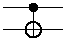
\includegraphics[scale=2]{img/CNOT_gate.pdf}
\vspace*{\fill}
\end{minipage}
\end{minipage}


\subsection*{EPR pairs}
The EPR pairs are the Bell states denoted by $\ket{\Phi ^+}$, $\ket{\Phi ^-}$, $\ket{\Psi ^+}$ and $\ket{\Psi ^-}$.
\vspace{2\baselineskip}

\begin{minipage}{\linewidth}
\begin{minipage}{0.5\linewidth}\center
$|\Phi^+\rangle = \frac{1}{\sqrt{2}} (|00\rangle_B + |11\rangle_B)$
\end{minipage}
\begin{minipage}{0.5\linewidth}\center
\vspace*{\fill}
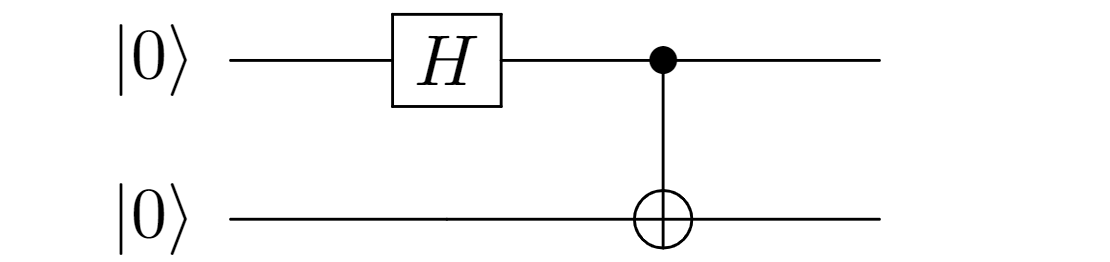
\includegraphics[scale=0.1]{img/h_cnot.png}
\vspace*{\fill}
\end{minipage}
\end{minipage}


\end{document}